\documentclass[12pt,a4paper]{article}
\usepackage{geometry}
\geometry{left=2.5cm,right=2.5cm,top=2.0cm,bottom=2.5cm}
\usepackage[english]{babel}
\usepackage{amsmath,amsthm}
\usepackage{amsfonts}
\usepackage[longend,ruled,linesnumbered]{algorithm2e}
\usepackage{fancyhdr}
\usepackage{ctex}
\usepackage{array}
\usepackage{listings}
\usepackage{color}
\usepackage{graphicx}
\usepackage{url}
\usepackage{hyperref}
\hypersetup{hidelinks}
\usepackage{longtable}
\usepackage{booktabs}
\usepackage{amsmath}
\usepackage{listings}

\lstset{
    basicstyle=\ttfamily\small,
    frame=single,
    breaklines=true,
    postbreak=\mbox{\textcolor{red}{$\hookrightarrow$}\space},
    showstringspaces=false,
    commentstyle=\color{gray},
    keywordstyle=\color{blue}
}

\begin{document}

\title{智能计算体系结构Lab1实验报告}
\date{}

\author{
姓名:\textbf{卞卓航}~~~~~~
学号:\textbf{22373017}~~~~~~
}

\maketitle

\section{实验目标}

本实验的目标是实现一个基本的多层神经网络,以支持简单的手写数字识别。

对于本实验提供了一个简单的三层神经网络,在两轮迭代的情况下可以达到97\%的正确率。这是一个很高的水平。基于提供的代码,我将其修改为了\textbf{深度可配置}的神经网络,并进行了一系列的实验。

并且,在实验过程中,我进一步学习了神经网络的相关知识,加深了对齐数学原理的认识。

\section{实验原理}

\subsection{神经元}

神经网络是由具有适应性的\textbf{简单单元组成的广泛并行互连的网络},它的组织能够模拟生物神经系统对真实世界物体所作出的交互反应。

M-P神经元模型:

\begin{itemize}
\item
  神经元接收到来自其他n个神经元传递过来的输入信号
\item
  这些输入信号通过\textbf{带权重的连接}进行传递。
\item
  神经元接收到的\textbf{总输入值将与神经元的阀值}进行比较
\item
  然后通过\textbf{激活函数}(activation function)处理以产生神经元的输出

  \begin{itemize}
  \item
    理想的激活函数是阶跃函数,将输入值映射为$\{0,1\}$,1代表神经元兴奋,0代表神经元抑制
  \item
    实际中会使用Sigmoid函数进行代替,也称为挤压函数
  \end{itemize}
\end{itemize}

事实上,从计算机科学的角度看,可以先不考虑神经网络是否真的模拟了生物神经网络,只需\textbf{将一个神经网络视为包含了许多参数的数学模型},这个模型是若干个函数,
例如$y_j=f(\sum_i w_i x_i -\theta_j)$相互(嵌套)代入而得到。

\subsection{反向传播}

对于BP算法,将误差进行反向传播,基于梯度下降的原理调整神经元的计算权重,实现更好的拟合效果。

\begin{enumerate}
\item
  先将输入示例提供给输入层神经元,逐层将信号前传,直到产生输出层的结果
\item
  然后计算输出层的误差,再将误差\textbf{逆向传播至隐层神经元}
\item
  最后根据隐层神经元的误差来对连接权和阈值进行调整
\item
  该法代过程循环进行,直到达到某些停止条件为止,输出连接权与阈值确定的多层前馈神经网络
\end{enumerate}

在数学上,由于采用的激励函数为$f(x) = \frac{1}{1 - e^{-x}}$,故有:

$$
f'(x) = f(x) (1 - f(x))
$$

进而在反向传播的梯度计算上,有:

\begin{equation}
\begin{aligned}
e_h &= - \frac{\partial E_k}{\partial b_h} \frac{\partial b_h}{\partial \alpha_h} \\
&= - \sum_{j = 1}^{l} \frac{\partial E_k}{\partial \beta_j} \frac{\partial \beta_j}{\partial b_h} f'(\alpha_h - \gamma_h) \\
&= b_h(1 - b_h) \sum_{j = 1}^{l} w_{hj} g_j 
\end{aligned}
\end{equation}


\section{实验实现}

在确定实验思路后,进行了相关代码的书写,实现了一个可配置层数的神经网络。

\subsection{神经网络结构调整}

在\texttt{model.py}文件中,将原先的单层隐藏层修改为了可配置深度的隐藏层。

为了进行简化,假定了每个隐藏层的神经元个数相同。

具体方式为:

\begin{enumerate}
\item
  修改隐藏层为一个列表\texttt{hidden\_outputs\_list},其中储存了隐藏层相关的输出信息
\item
  将隐藏层的权重信息修改为列表形式的\texttt{whh\_list},其中的\texttt{whh\_list{[}i{]}}表示第\texttt{i}个隐藏层和第\texttt{i+1}个隐藏层之间的权重信息。其初始值均在网络初始化时进行随机初始化。
\end{enumerate}

\subsection{前向传播}

前向传播的思路与原先类似。通过循环的方式实现了对隐藏层的逐层计算,达成了整体的前向传播。

\begin{lstlisting}
# 计算输入层
self.inputs = np.array(input_feature, ndmin=2).T

# 计算相邻的隐藏层
hidden_inputs = np.dot(self.wih, self.inputs)
for i in range(self.hidden_depth):
    self.hidden_outputs_list[i] = self.activation_function(hidden_inputs)
    hidden_inputs = np.dot(self.whh_list[i - 1], self.hidden_outputs_list[i])

# 计算输出层
final_inputs = np.dot(self.who, self.hidden_outputs_list[self.hidden_depth - 1])
self.final_outputs = self.activation_function(final_inputs)
\end{lstlisting}

\subsection{反向传播}

反向传播需要修改代码的两个部分:

\begin{lstlisting}
# hidden layer error
hidden_error = [None for _ in range(self.hidden_depth)]
hidden_delta = [None for _ in range(self.hidden_depth)]

# calculate hidden layer error and delta
for i in reversed(range(self.hidden_depth)):
    if i == self.hidden_depth - 1:
        hidden_error[i] = np.dot(self.who.T, output_delta)
        hidden_delta[i] = hidden_error[i] * self.hidden_outputs_list[i] * (1.0 - self.hidden_outputs_list[i])
    else:
        hidden_error[i] = np.dot(self.whh_list[i - 1].T, hidden_delta[i + 1])
        hidden_delta[i] = hidden_error[i] * self.hidden_outputs_list[i] * (1.0 - self.hidden_outputs_list[i])
\end{lstlisting}

\begin{enumerate}
\item
  实现对每一层的误差计算
\item
  在计算误差后,需要遍历所有的隐藏层,计算相应的梯度,进行反向传播
\end{enumerate}

为了进行一定的简化,之前假定了各隐藏层的神经元个数相同,因此每一层的计算形式是相同的,只需要通过循环遍历每一个隐藏层即可:

\section{实验结果与分析}

在实现了\textbf{可配置层数}的多层神经网络后,对实验相关的神经网络层数、学习率、中间节点数、迭代轮数都进行了相关的实验。

\subsection{实验结果}

其中实验结果为:

\begin{longtable}{c c c c c}
\caption{实验结果} \\
\toprule
层数 & 学习率 & 中间节点数 & 迭代轮数 & 准确率 \\
\endfirsthead

\multicolumn{5}{c}%
{{\bfseries \tablename\ \thetable{} -- 续前页}} \\
\toprule
层数 & 学习率 & 中间节点数 & 迭代轮数 & 准确率 \\
\endhead

\bottomrule
\endfoot

\midrule
\endfoot

3 & 0.1 & 200 & 2 & 97 \\
4 & 0.1 & 200 & 2 & 91 \\
5 & 0.1 & 200 & 2 & 51 \\
6 & 0.1 & 200 & 2 & 10 \\
7 & 0.1 & 200 & 2 & 10 \\
102 & 0.1 & 200 & 2 & 10 \\
3 & 0.1 & 200 & 10 & 97.42 \\
4 & 0.1 & 200 & 10 & 97.22 \\
5 & 0.1 & 200 & 10 & 95.08 \\
6 & 0.1 & 200 & 10 & 67.09 \\
7 & 0.1 & 200 & 10 & 9.74 \\
4 & 0.1 & 200 & 2 & 93.96 \\
4 & 0.2 & 200 & 2 & 93.26 \\
4 & 0.3 & 200 & 2 & 93.58 \\
4 & 0.4 & 200 & 2 & 91.59 \\
4 & 0.5 & 200 & 2 & 83.94 \\
4 & 0.1 & 100 & 2 & 88.37 \\
4 & 0.1 & 200 & 2 & 93.94 \\
4 & 0.1 & 300 & 2 & 93.56 \\
4 & 0.1 & 400 & 2 & 93.93 \\
4 & 0.1 & 500 & 2 & 93.32 \\
\end{longtable}

\subsection{实验结果分析}

\subsubsection{神经网络深度}

首先,在其他参数与baseline保持相同的情况下,调整了神经网络的层数,从实验结果中可以看出,当层数为3、4、5时,依然具有较好的识别效果,但是当层数为6时,识别率急速下降,识别率仅有0.118,显著小于其他参数设置下的0.9以上的识别率。

对此总结为:当迭代轮数较少而神经网络较深时,可以看到神经网络的分类效果极低,没有达到训练效果。

\begin{figure}[htbp]
    \centering
    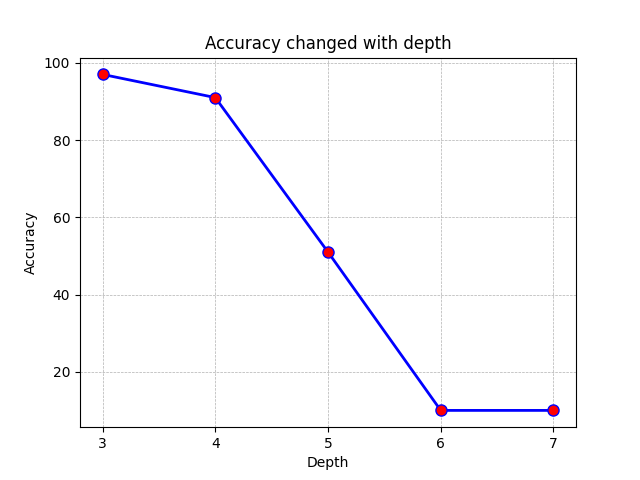
\includegraphics[width=0.5\linewidth]{img/accuracy-depth.png}
    \caption{accuracy-depth}
\end{figure} 

通过对神经网络的分析,推测其可能的原因是为当轮数较少时,相关权重依然处于一个较为随机的状态,反向传播的调整并没有起到很好的作用。整体网络依然以一种近乎于初始随机状态的效果进行运行。

同时,还训练了一个100层的神经网络,在epoch=2和epoch=200的情况下训练效果均较差。限于本次实验要求不使用框架,未使用\texttt{pytorch}进行进一步的尝试。

\subsubsection{训练迭代轮数}

为了上述猜想,在其他参数保持不变的情况下,将实验的迭代轮数调整为了10,观察此次的训练效果,发现有了较为显著的提升。

对此,可以进行一定的总结:当神经网络深度较深时,训练轮数较少会使得神经网络没有较好的效果,反而不如深度较低的情况。

\begin{figure}[htbp]
    \centering
    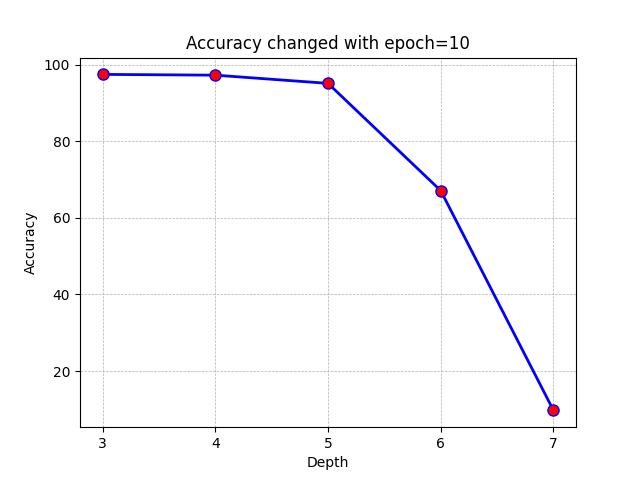
\includegraphics[width=0.5\linewidth]{img/accuracy-epoch.png}
    \caption{accuracy-epoch}
\end{figure} 

\subsubsection{改变学习率}

在相较于baseline其他情况不变的情况下,修改了不同的学习率,发现学习率也会对实验造成一定的影响。

\begin{figure}[htbp]
    \centering
    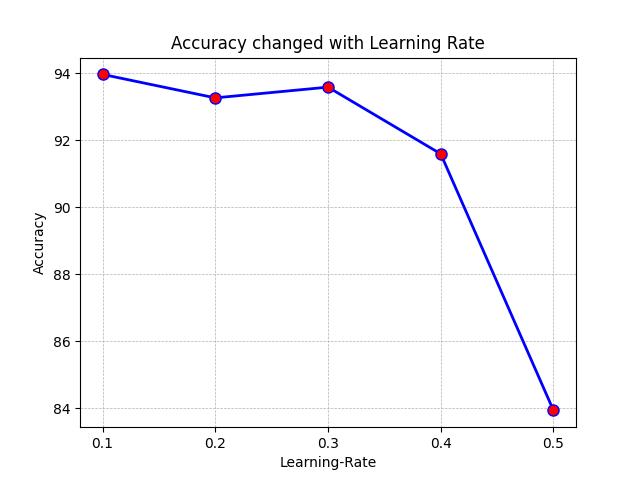
\includegraphics[width=0.5\linewidth]{img/accuracy-lr.png}
    \caption{accuracy-lr}
\end{figure} 

\subsubsection{改变中间节点数目}

在相较于baseline其他情况不变的情况下,修改了不同的隐藏层节点数,发现中间节点数目也会对实验造成一定的影响。

\begin{figure}[htbp]
    \centering
    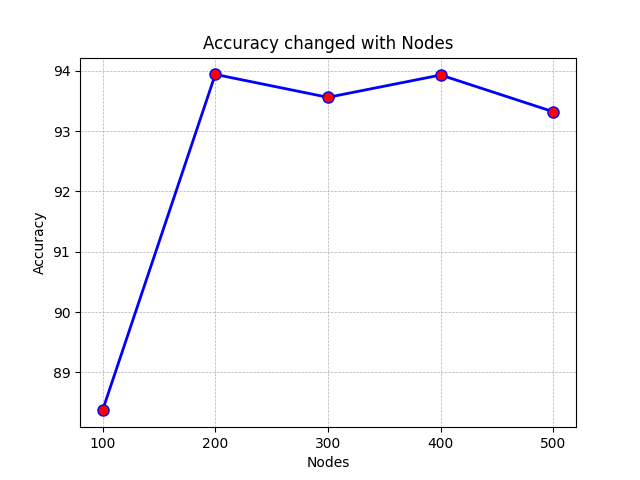
\includegraphics[width=0.5\linewidth]{img/accuracy-nodes.png}
    \caption{accuracy-nodes}
\end{figure} 

\section{实验总结}

在本次实验中,完成了对简单DNN的修改,进行了各种参数的修改,观察了不同的训练效果。

在本次实验中,我加深了对反向传播的理解。

\end{document}